\subsubsection{Robustness for a low-cost device}
\label{sec:res-robust}

Four tests (\vn{crossing_ml_robust.m}, Section~\ref{sec:analyses}) ask whether the device result survives cheaper hardware and a
small processor. The sampling-rate and noise tests use six features per signal for two settings: a real-time cue from the leading
limb up to 0.3\,s before the trailing lift-off (80.1\,\% at 60\,Hz) and the result after the crossing from both limbs (89.2\,\%).
Figure~\ref{fig:robust} summarises them.

\paragraph{Sampling rate.} From 60 to 10\,Hz the accuracy drops by 2.6 points for the real-time cue (80.1 to 77.4\,\%) and by
2.3 points after the crossing (89.2 to 86.9\,\%); no rate costs more than 3.1 points (Table~\ref{tab:robrate}). The obstacle is
written in slow movements (foot lift, thigh and shank tilt over 0.2--0.5\,s), so a 10--20\,Hz stream keeps it. The foot height was
still integrated at 60\,Hz; a less accurate integration at a low IMU rate is not simulated.

\paragraph{Sensor noise.} With the noise of a good IMU (1--2\textdegree{} tilt, 0.25--0.5\,m/s$^2$ acceleration, 5--10\,mm foot
height) the accuracy does not change ($-0.3$ to $+1.0$ points); only at 8\textdegree{} and 40\,mm does it fall, to 76.5\,\% for
the real-time cue and 87.7\,\% after the crossing (Table~\ref{tab:robnoise}). The features are maxima, minima and means over many
samples, which average the noise. A constant offset, such as a sensor mounted a few degrees off, is removed by both the level-walk
calibration and the person scaling.

\paragraph{Model size.} The device model (300 trees, minimum leaf 2) reaches 92.3\,\% and needs about 311\,kB
(Table~\ref{tab:robforest}). Ten trees with a minimum leaf of 30 reach 91.2\,\% in about 3\,kB, small enough for a
microcontroller. A logistic model with a single feature per limb, most often the peak height of the leading foot and the height of
the trailing foot at 25\,\% of its swing, reaches 89.2\,\% in 72 bytes, and with two features per limb 90.8\,\% in 120 bytes
(Table~\ref{tab:roblogistic}); more features do not help the logistic model (86.1--89.3\,\%).

\paragraph{Prediction sets.} Instead of a single height, the device can return the set of plausible heights with a guaranteed
coverage for a new person (split-conformal, Table~\ref{tab:robconformal}). At a 90\,\% target the sets contain the true height in
91.2\,\% of the crossings (H1 94\,\%, H2 88\,\%, H3 91\,\%): 97.7\,\% of the crossings get a single height and 2.3\,\% an empty
set (no cue), and the 8.8\,\% not covered are 6.5\,\% wrong single heights and the 2.3\,\% empty sets. At 95\,\% the coverage is
94.6\,\% and 14.6\,\% of the sets are two neighbouring heights; H1 and H3 together, or all three heights, never occur. At 80\,\%
the sets are empty for 16.2\,\% of the crossings. A cue can therefore name one height, fall back to ``one of two neighbouring
heights'' at a strict target, and stay silent when no height is plausible enough.

\begin{table}[htbp]
\centering
\caption{Sampling rate: balanced accuracy (95\,\% CI) when every signal is averaged over its last $m$ samples and decimated from
60\,Hz to 30, 20, 15 and 10\,Hz.}
\label{tab:robrate}
\begin{adjustbox}{max width=\textwidth}
{\footnotesize
\begin{tabular}{p{4.4cm}rrrrr}
\toprule
\textbf{setting} & \textbf{60 Hz} & \textbf{30 Hz} & \textbf{20 Hz} & \textbf{15 Hz} & \textbf{10 Hz} \\
\midrule
real-time cue: leading limb up to 0.3 s before the trailing lift-off & 80.1\% (72--88) & 81.6\% (74--89) & 80.4\% (71--88) & 77.0\% (68--85) & 77.4\% (68--85) \\
after the crossing: both limbs, $-$1.5 to +0.6 s & 89.2\% (85--93) & 88.8\% (83--94) & 88.4\% (83--93) & 88.4\% (84--93) & 86.9\% (82--91) \\
\bottomrule
\end{tabular}
}
\end{adjustbox}

\end{table}

\begin{table}[htbp]
\centering
\caption{Sensor noise: mean balanced accuracy over three draws of independent Gaussian noise added to every sample (min--max in
brackets).}
\label{tab:robnoise}
\begin{adjustbox}{max width=\textwidth}
{\scriptsize
\begin{tabular}{p{3.4cm}rrrrr}
\toprule
\textbf{setting} & \textbf{none} & \textbf{1 deg / 0.25 m/s$^2$ / 5 mm} & \textbf{2 deg / 0.5 m/s$^2$ / 10 mm} & \textbf{4 deg / 1 m/s$^2$ / 20 mm} & \textbf{8 deg / 2 m/s$^2$ / 40 mm} \\
\midrule
real-time cue: leading limb up to 0.3 s before the trailing lift-off & 80.1\% (80--80) & 80.8\% (80--82) & 81.1\% (79--83) & 80.3\% (77--83) & 76.5\% (75--77) \\
after the crossing: both limbs, $-$1.5 to +0.6 s & 89.2\% (89--89) & 88.8\% (88--90) & 89.2\% (88--90) & 88.5\% (87--90) & 87.7\% (87--89) \\
\bottomrule
\end{tabular}
}
\end{adjustbox}

\end{table}

\begin{table}[htbp]
\centering
\caption{Model size, random forests of the device model: balanced accuracy and memory (12 bytes per tree node, both limbs).}
\label{tab:robforest}
\begin{adjustbox}{max width=\textwidth}
{\scriptsize
\begin{tabular}{lrrrrrr}
\toprule
\textbf{forest} & \textbf{5 trees} & \textbf{10 trees} & \textbf{25 trees} & \textbf{50 trees} & \textbf{100 trees} & \textbf{300 trees} \\
\midrule
minimum leaf 2 & 90.7\% (5 kB) & 89.5\% (10 kB) & 90.7\% (26 kB) & 90.2\% (52 kB) & 92.2\% (103 kB) & 92.3\% (311 kB) \\
minimum leaf 10 & 86.5\% (3 kB) & 90.4\% (6 kB) & 90.4\% (14 kB) & 91.6\% (27 kB) & 91.9\% (55 kB) & 91.2\% (166 kB) \\
minimum leaf 30 & 88.9\% (1 kB) & 91.2\% (3 kB) & 90.4\% (6 kB) & 92.0\% (13 kB) & 90.9\% (25 kB) & 90.5\% (76 kB) \\
\bottomrule
\end{tabular}
}
\end{adjustbox}

\end{table}

\begin{table}[htbp]
\centering
\caption{Model size, logistic regression with the $k$ best features per limb (chosen inside each training set): balanced accuracy
and memory.}
\label{tab:roblogistic}
\begin{adjustbox}{max width=\textwidth}
{\scriptsize
\begin{tabular}{lrrrrrrr}
\toprule
\textbf{logistic} & \textbf{k = 1} & \textbf{k = 2} & \textbf{k = 3} & \textbf{k = 5} & \textbf{k = 10} & \textbf{k = 20} & \textbf{all features} \\
\midrule
balanced accuracy (memory) & 89.2\% (72 B) & 90.8\% (120 B) & 89.3\% (168 B) & 88.9\% (264 B) & 86.5\% (504 B) & 86.1\% (984 B) & 86.4\% (2 kB) \\
\bottomrule
\end{tabular}
}
\end{adjustbox}

\end{table}

\begin{table}[htbp]
\centering
\caption{Conformal prediction sets: observed coverage overall and per class, mean set size, and share of the crossings by set
type (in brackets: single height and right).}
\label{tab:robconformal}
\begin{adjustbox}{max width=\textwidth}
{\scriptsize
\begin{tabular}{rrp{3.0cm}rrrrrr}
\toprule
\textbf{target coverage} & \textbf{observed coverage} & \textbf{per class} & \textbf{mean set size} & \textbf{one class (right)} & \textbf{two neighbouring classes} & \textbf{H1 + H3 only} & \textbf{all three} & \textbf{empty} \\
\midrule
80\% & 80.8\% & H1 92\%, H2 73\%, H3 77\% & 0.84 & 83.8\% (80.8\%) & 0.0\% & 0.0\% & 0.0\% & 16.2\% \\
90\% & 91.2\% & H1 94\%, H2 88\%, H3 91\% & 0.98 & 97.7\% (91.2\%) & 0.0\% & 0.0\% & 0.0\% & 2.3\% \\
95\% & 94.6\% & H1 99\%, H2 92\%, H3 93\% & 1.14 & 85.0\% (80.4\%) & 14.6\% & 0.0\% & 0.0\% & 0.4\% \\
\bottomrule
\end{tabular}
}
\end{adjustbox}

\end{table}

\begin{figure}[htbp]
\centering
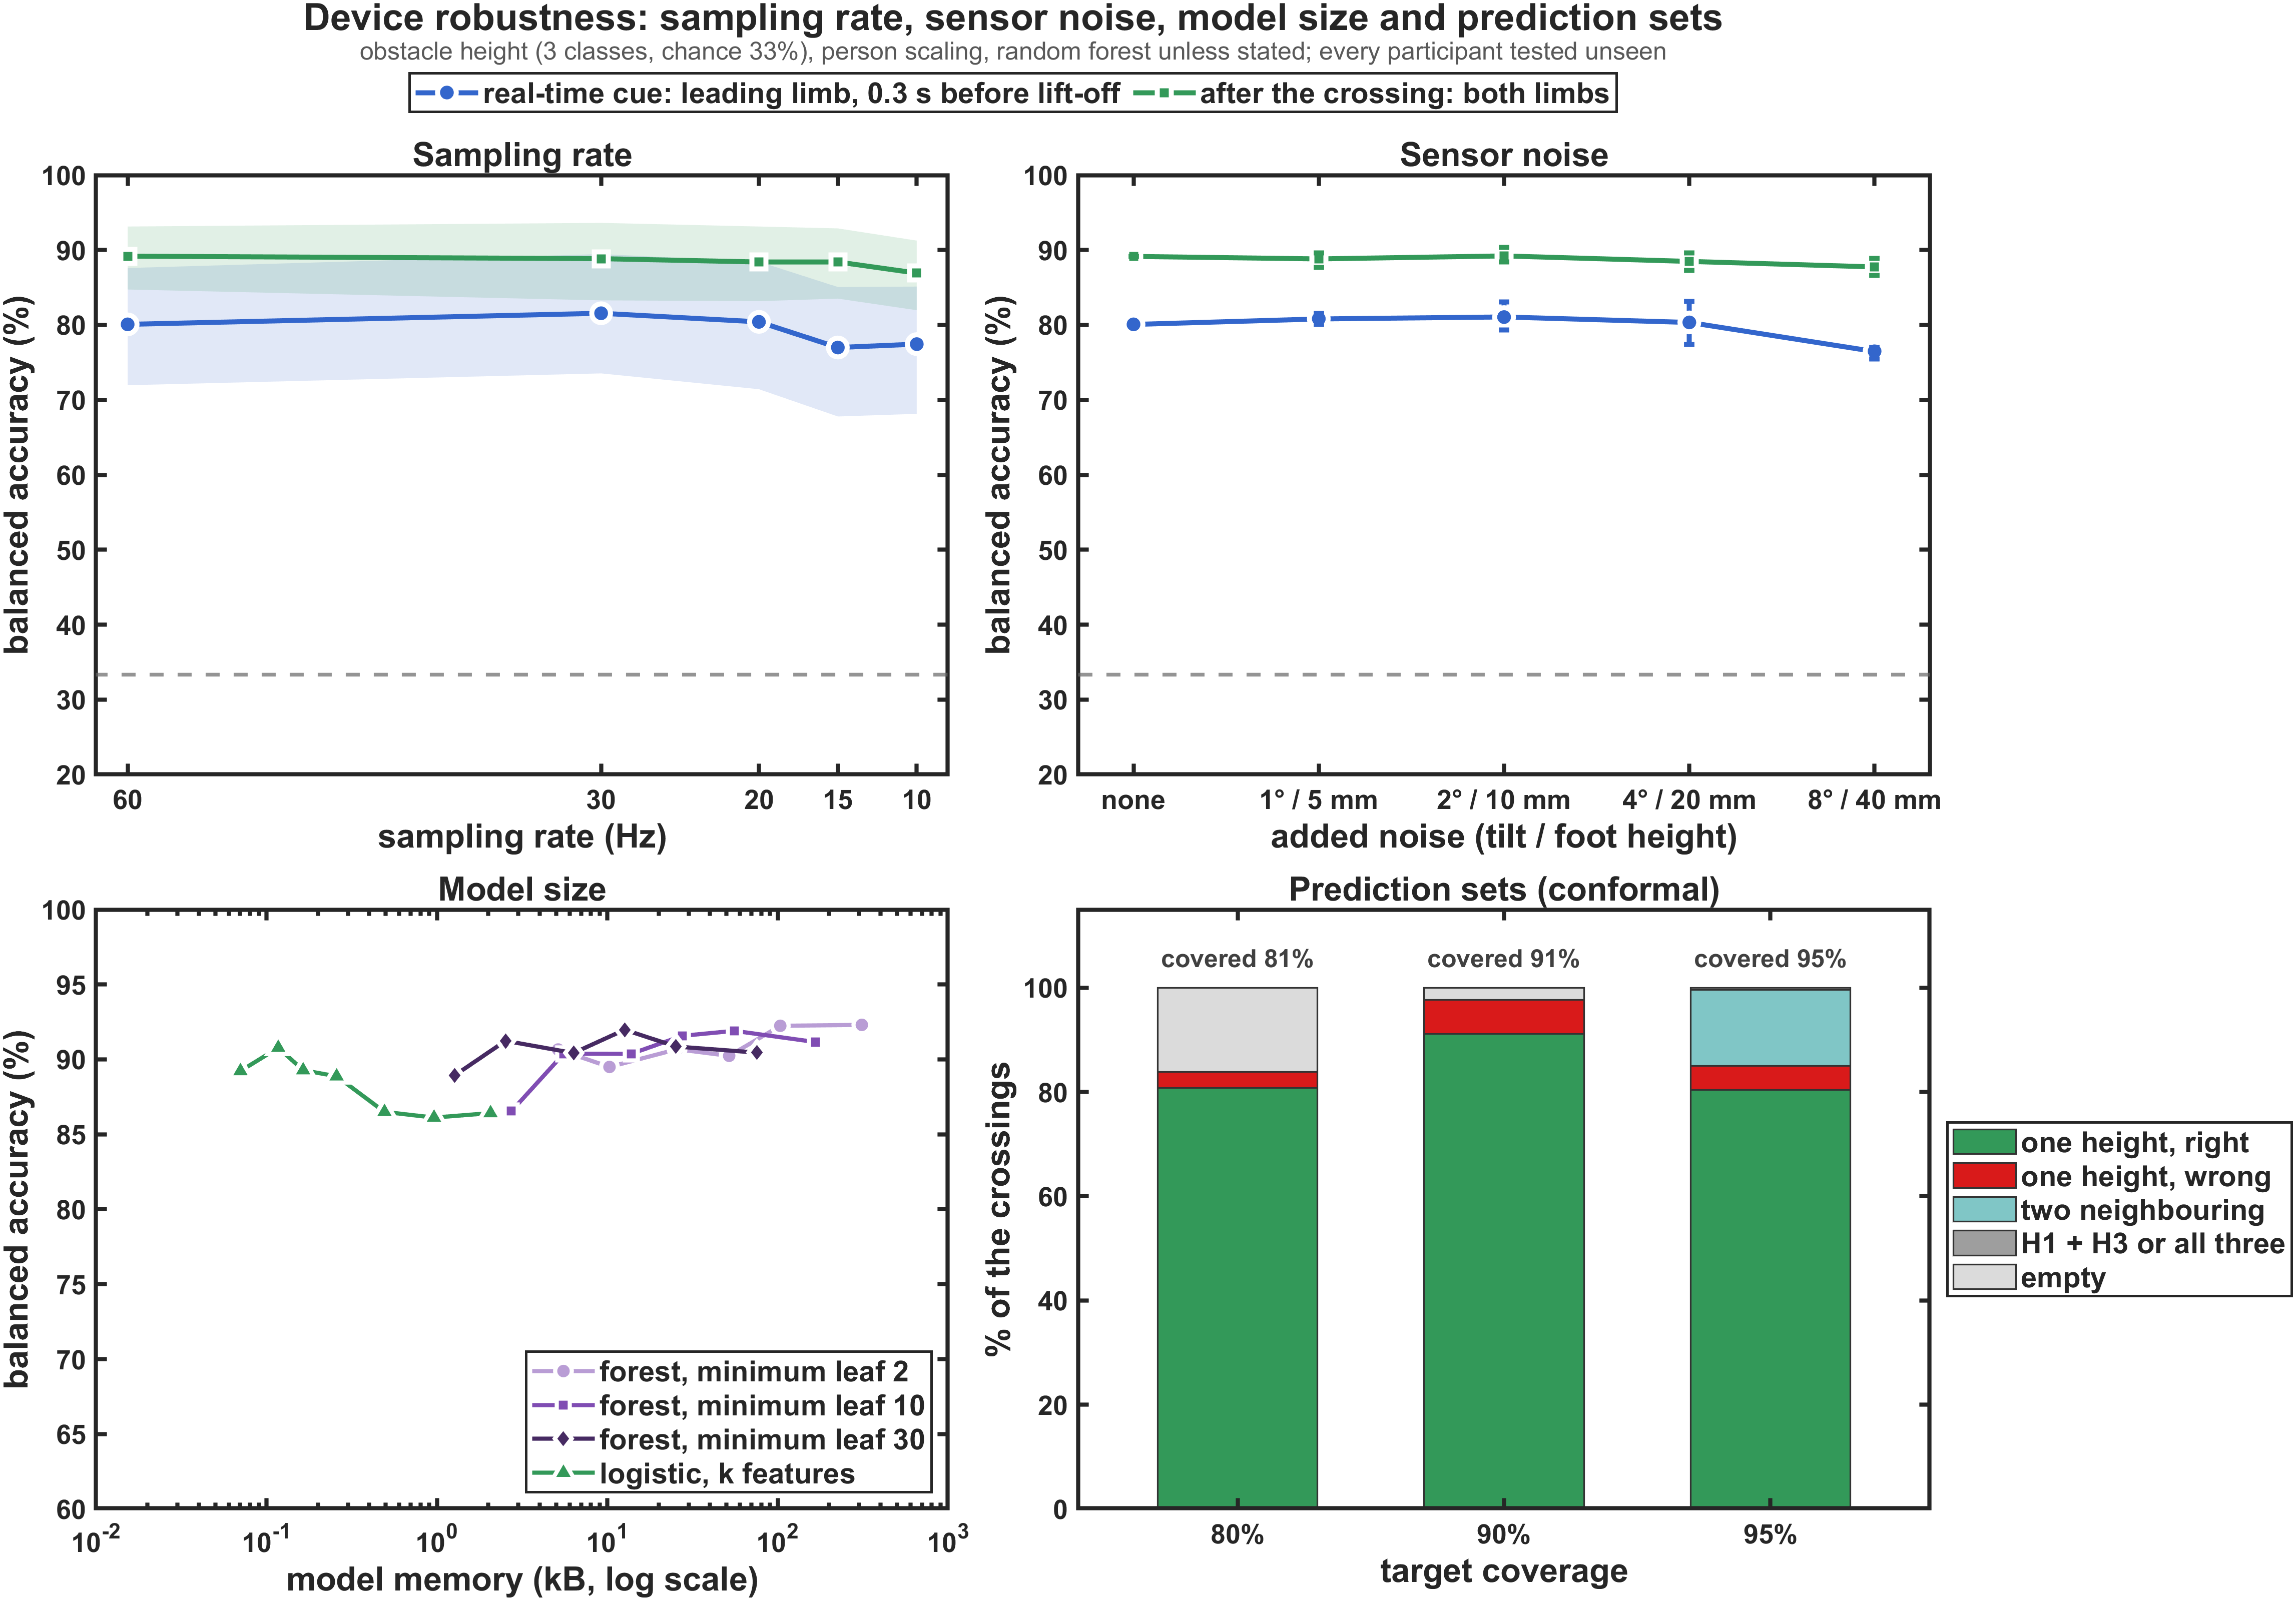
\includegraphics[width=\textwidth]{fig_robust.png}
\caption{Device robustness. Top left: balanced accuracy against the sampling rate for the real-time cue (blue: leading limb up to
0.3\,s before the trailing lift-off) and after the crossing (green: both limbs); band = 95\,\% participant-bootstrap CI. Top right:
against added sensor noise (mean and min--max over three draws). Bottom left: against model memory for forests (purple, minimum
leaf 2, 10 and 30; 5--300 trees) and logistic models with the $k$ best features per limb (green). Bottom right: conformal
prediction sets at 80, 90 and 95\,\% target coverage: one right height (green), one wrong height (red), two neighbouring heights
(light teal), H1 + H3 or all three (grey) and empty (light grey); observed coverage above the bars. Dashed = chance.}
\label{fig:robust}
\end{figure}
